

\section{Introduction}
\label{sec:introduction}

The ability to compare methods is an important aspects of further development of that method. In the case of attack trees, the ability to compare attack trees is critical for the sharing of threat intelligence. Attack trees are a method of modeling threats, and are used in a variety of industries, including cybersecurity, physical security, and safety analysis. However, there is no standard method for comparing attack trees. In this paper, we propose a method for comparing attack trees, and define a set of distance measures for comparing attack trees. We then apply these distance measures to a dataset of attack trees, and show how they can be used to compare attack trees.

Our primary research goal is to determine a mechanism to calculate the distance between two attack trees. This is a novel problem, as a distance measure between attack trees has not been established. Further, a means of experimentally validating a distance measures has yet to be established.


\subsection{Research Questions and Contributions}


Our fundamental research question is: \emph{How do we measure the distance between two attack trees?}

To answer this, we start by understanding the requirements behind measure distance metric, based on our experience with attack trees and related literature. We then propose a repeatable method for experimentally validating any tree distance metric. We further propose both a mechanism for processing different node labels with similar meanings and novel algorithms for calculating the distance between two attack trees. Finally, combine all of this to propose a distance function that behaves in a reasonable and intuitive manner.

% - start understanding requirements, propose a way to experimentally validate any distance metric, then we propose the semantic similarity idea, and then we have collected a set of metrics based on attack tree and tree distance literature. We are able to propose a function that behaves in a somewhat reasonable way
% - Main research question: How do we measure the distance between two attack trees?

% We posit the following research questions:

% \begin{enumerate}
%     \item[\RQ{1}] How can we best calculate the distance between two attack trees?
% \item[\RQ{2}] Is this method of attack tree distance valid?
% \end{enumerate}

\subsection{Motivation}

% \textit{This subsection may be removed in the final paper, but it helps to frame why we are doing this}.

Threat modeling seeks to organize threat information that aids in comprehension and analysis~\cite{andersonSecurityEngineeringGuide2020,schneierSecretsLiesDigital2000}. Many attack trees are drawn by practitioners in the course of their work. However, most attack trees at the moment exist in a vacuum, they are created for a specific team or practitioner with diminished value beyond this scope. By developing a methodology for calculating the distance (or difference) between two attack trees, we can empower practitioners with a simple mechanism to compare their attack trees with those of others. This could be used to find attack trees that are similar, with the differences representing missing components and attack vectors, or to find differences in analysis. Given the increasing prevalence of LLMs and the application of LLMs to a wider array of fields, being able to compare self drawn attack trees to a large collection of machine generated attack trees would be a powerful tool for practitioners. Further, defining a repeatable method for experimentally validating a distance measure will enable others to further refine our work or develop new distance measures that are comparable to those we provide.



%%%%%%%%%%%%%%%%%%%%%%%%%%%%%%%%%%%%%%%%%%%%%%%%%%%%%%%%%%%%%%%%%%%%%%%%%%%%%%%%%%%%%%%%%%%%%%%%%


\section{Background}
\label{sec:background}


% \begin{figure*}
%     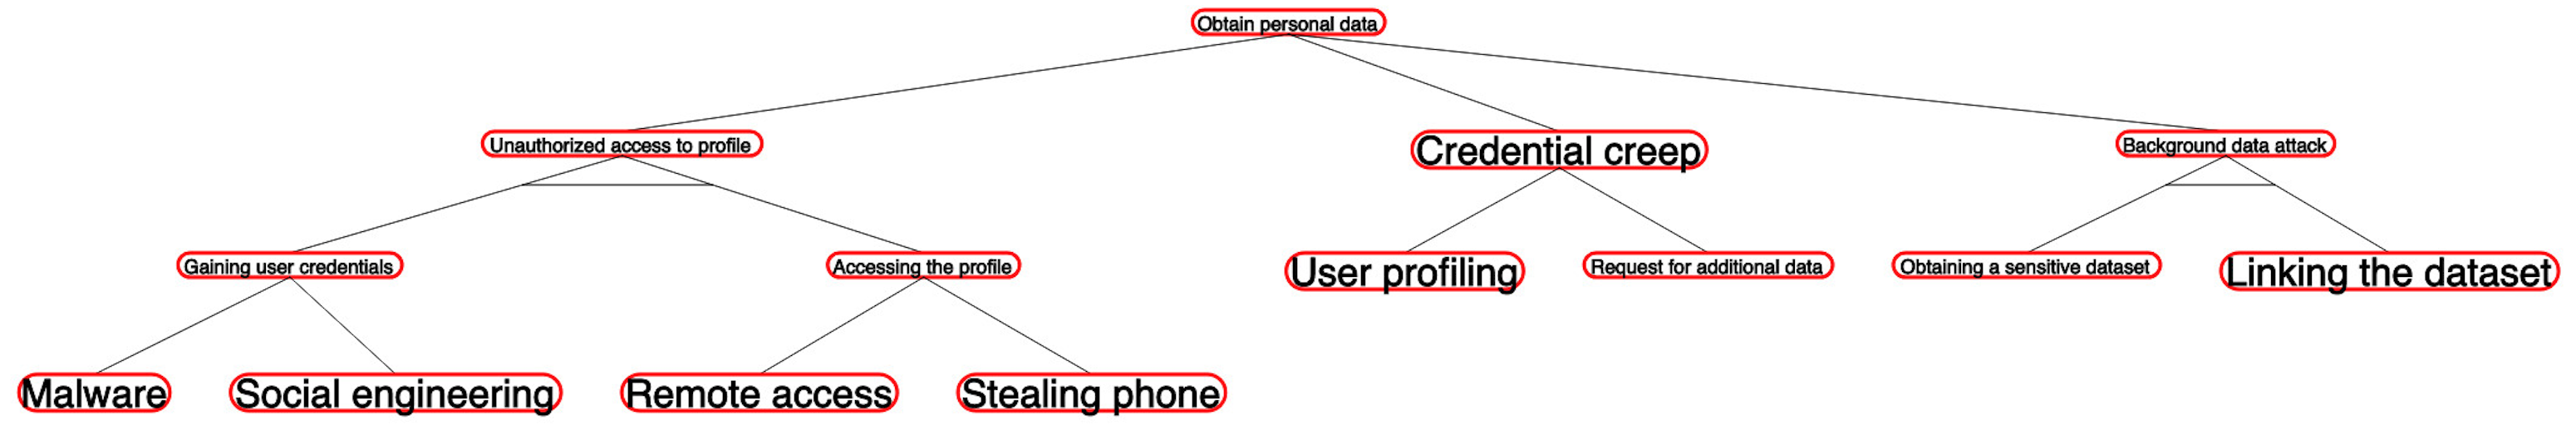
\includegraphics[width=\linewidth]{img/TargetAT.png}
%     \caption{An attack tree adapted from Naik \etal~\cite{naikEvaluationPotentialAttack2022} that is used in the study described in Section~\ref{sec:methodology}. }
%     \label{fig:tartgetAT}
% \end{figure*}



\begin{figure*}
\resizebox{\linewidth}{!}{
    \begin{forest}
        for tree={
        draw,
        minimum height=.25cm,
        anchor=parent,
        align=center,
        child anchor=parent,
        edge=-
        },
        adnode/.style={rounded rectangle,},
        [{Obtain personal data}, adnode,
                [{Unauthorized access to profile}, adnode, small angle below,  [{Gaining user credentials}, adnode,[{Malware}, adnode,][{Social engineering}, adnode,]] [{Accessing the profile}, adnode,[{Remote access}, adnode,][{Stealing phone}, adnode,]]]
                    [{Credential creep}, adnode,  [{User profiling}, adnode,] [{Request for additional data}, adnode,]]
                    [{Background data attack}, adnode, small angle below, [{Obtaining a sensitive dataset}, adnode,] [{Linking the dataset}, adnode,]]
            ]
    \end{forest}
}
\caption{An attack tree adapted from Naik~\etal~\cite{naikEvaluationPotentialAttack2022} that is used in the study described in Section~\ref{sec:methodology}. }
    \label{fig:tartgetAT}
\end{figure*}

% \begin{figure*}
%     \resizebox{\linewidth}{!}{
%         \begin{forest}
%             for tree={
%             draw,
%             minimum height=.25cm,
%             anchor=parent,
%             align=center,
%             child anchor=parent,
%             edge=-
%             },
%             adnode/.style={rounded rectangle,},
%             [{Obtain personal data}, adnode,
%                     [{Unauthorized profile access}, adnode, small angle below,
%                             [{Gaining user cred.}, adnode,
%                                     [{Malware}, adnode,]
%                                         [{Social engineering}, adnode,]]
%                                 [{Access profile}, adnode,
%                                     [{Remote access}, adnode,]
%                                         [{Steal phone}, adnode,]]]
%                         [{Background data attack}, adnode, small angle below,
%                             [{Obtain dataset}, adnode,]
%                                 [{Link dataset}, adnode,]]
%                         [{Cred. creep}, adnode,
%                             [{User profiling}, adnode,]
%                                 [{Request additional data}, adnode,]]
%                 ]
%         \end{forest}
%     }
%     \caption{An attack tree that was also adapted from Naik~\etal~\cite{naikEvaluationPotentialAttack2022} which should be equivalent to Figure~\ref{fig:tartgetAT}. This will be used in Section~\ref{sec:distance} to model the different distance measurements.}
%     \label{fig:tartgetAT2}
% \end{figure*}

We define attack trees, as initially described by Bruce Schneier~\cite{schneierAttackTrees1999}, to be a rooted acyclic structure with the following recursive definition  from Gadyatskaya~\etal~\cite{gadyatskayaRefinementAwareGenerationAttack2017}.

\begin{definition} \label{def:attack-tree}

An attack tree $t$ is defined as:
\[
    t = b | b\Delta(t_1, ..., t_i)
\]

Where $b \in \mathbb{B}$ is an action or goal in service of an attack, where $\mathbb{B}$ is the set of all possible attack components. For our purposes, $b$ is considered the label of a node. $\Delta$ is the refinement of a node, giving the relationship between child nodes. For our purposes, $\Delta$ is either \AND\ or \OR.



% An attack tree  is defined as $T = \ATnode{1}{1}\Delta(\ATnode{2}{1},...,\ATnode{2}{i})$. Where $\ATnode{d}{i} = \ATlabel{d}{i}\Delta(\ATnode{d+1}{j},...,\ATnode{d+1}{k})$

    % We define the $i\text{th}$ node according to left-right post-order number to be the following, $T[i] = b\Delta(T[j],...,T[k])$. 

    % We give $b$ to be some action within the attack scenario, which is the node label of $t$. For clarity, we additionally refer to this label as $t.\text{label}$. We give $\Delta$ to be the refinement $\Delta = \AND|\OR|\SAND$. For clarity and consistency, we refer to the refinement of a given node to be $t.\Delta$. Following the refinement, we have a list of nodes which are the children of $t$, defined as $t_0,...,t_i$ which is the left to right order of the children (regardless of if order is significant). We refer to the list of children as $t.\text{children}$. This list of nodes can be empty, in the case of leaf nodes.

    % For clarity and consistency, we refer to the refinement of a given node to be $t.\Delta$. Following the refinement, we have a list of nodes which are the children of $\ATnode{d}{i}$, defined as $\ATnode{d+1}{j},...,\ATnode{d+1}{k}$ where $j \ge 1$ and $k \ge j$, which is the left to right order of the children (regardless of if order is significant). We refer to the list of children as $\ATnode{d}{i}.\text{children}$. This list of nodes can be empty, in the case of leaf nodes.

% Each node within an attack tree is a sub-tree unto itself. We define each node as $\ATnode{d}{i}$ where $d$ is the depth of the node (distance from the root, given the root has a starting distance of 1), and $i$ is the number of that node counting from the left most node at depth $d$ (starting from 1). We define a mapping of each node to a label space, where the label of node $\ATnode{d}{i}$ is given as $\ATlabel{d}{i}$. We give $\Delta$ to be the refinement $\Delta = \AND|\OR$. We further define the following functions to retrieve associated information of some node $\ATnode{d+1}{j}$. We define the $\Delta(\ATnode{d}{i})$ function to return the refinement of a given node. We define the child function, $\childFunc{\ATnode{d}{i}}$ to return a list of nodes which are the children of a given node, defined as $\ATnode{d+1}{j},...,\ATnode{d+1}{k}$ where $j \ge 1$ and $k \ge j$, which is the left to right order of the children (regardless of if order is significant). This list of nodes can be empty, in the case of leaf nodes. Finally, we define the parent function, $\parentFunc{\ATnode{d}{i}}$ to return the parent of a given node.
\end{definition}

Fundamentally, distance measures provide a means of comparison, and means of comparison are critical for any industry. New applications of distance measures are easily found once the distance measure to defined~\cite{beham2011new}. We propose two potential uses of these distance measures; however, future work will further specify new applications. Threat models are a recommended tool for threat analysis~\cite{andersonSecurityEngineeringGuide2020,schneierSecretsLiesDigital2000}. However, once these models are created, they may only be applicable to the analyst or the team of analysts that created them. Unlike other sources of threat intelligence, such as YARA Rules~\cite{naik2019cyberthreat,naik2020evaluating}, there is no means to share attack trees in this format.

In order to allow for attack trees to be shared as threat intelligence, two aspects are needed: a common structure and a means of comparison. The common structure has already been defined, in the ADTool XML Schema~\cite{kordy_adtool_2013}. This is an XML format used by ADTool, a tool to create Attack-Defense Trees, an extension of ATs. The ADTool XML Schema can be used to define attack trees, and as such, can be used as a common structure for sharing attack trees. The dataset of ATs we describe in Section~\ref{sec:results} is in this format. The second aspect is a means of comparison, which is what we have defined in this paper. It will be possible to publish attack trees in the ADTool XML Schema, and then compare the resulting trees using the distance measures we have defined. This will allow for the sharing of attack trees as threat intelligence, and the comparison of these trees to identify similar threats.

% \subsubsection{Generative AI}

% Applying generative AI to security is an active area of research. Distance measures are critical for using generative AI to create threat models in general, and attack trees specifically. By using a distance measure, we can compare the output of a generative AI to a set of known attack trees, and determine how similar the output is to the known attack trees. As we can control the form of the output of generative AI, we can have an AI tool output AT in the ADTool XML Schema, and then compare the resulting attacks to our own output or to a dataset.

% Going further, in order to build and refine a generative AI tool to create attack trees, most method will require a cost function to be defined~\cite{bottou1991stochastic}. A cost function is necessary for most model training, as this is what the model will attempt to optimize for. Fundamental to this cost function is the ability to define distance, as we can offer a way to compare a generated solution to a ``ground truth''. Beyond this, distance measures can be used to better define which and how artificial intelligence systems should be applied to attack trees, as was shown by Terry Jones~\cite{jones1995fitness}.
